\documentclass[tp]{lcc}

% add latex preamble
% para la bibliografía se requiere biber y configurar texstudio

% Latex packages
\usepackage[utf8]{inputenc}
\usepackage[T1]{fontenc} % para copiar acentos en español del pdf y permite acentos en las notas
\usepackage[spanish]{babel}
\usepackage[per-mode = symbol]{siunitx} % para manejar las unidades
\usepackage{multimedia} % to add videos with \movie command
\usepackage{multirow}
\usepackage{graphicx}
\usepackage{xcolor}
\usepackage{amsmath} % bmatrix
\usepackage[makeroom]{cancel} % \cancel to cancel terms in math equations
\renewcommand{\CancelColor}{\color{red}} % set red color for \cancel command
\usepackage[caption=false]{subfig} % caption = false elimina la palabra "Figura" del caption
\usepackage{import} % para el comando import (se usa para pdf_tex)
\captionsetup[subfigure]{labelformat=empty} % remover el indice del caption de la subfigura
\usepackage{booktabs} % \toprule \midrule \bottomrule
\usepackage[backend=biber]{biblatex} % set biber to format references. Must configure Biber in Texstudio
\usepackage{csquotes} % to remove warning triggered by biblatex and babel
\usepackage{algorithm} % to put captions to the algorithmics environmets
\usepackage{algpseudocode} % to write algorithm
\usepackage{tikz} % to use tikz
\usetikzlibrary{fit} % to fit a node around other nodes in tikz
\usepackage[export]{adjustbox} % valign in subfloat
\usepackage{colortbl} % to paint cells in a table

% Color commands for annotations
\newcommand\TODO[1]{\textbf{\textcolor{red}{#1}}} %  TODO notes

% Graphic paths
\graphicspath{{./images/}}

% listings configuration for C code
\usepackage{listings} % code
\definecolor{commentgreen}{RGB}{2,112,10}
\definecolor{eminence}{RGB}{108,48,130}
\definecolor{weborange}{RGB}{255,165,0}
\definecolor{frenchplum}{RGB}{129,20,83}

\lstset{ % spanish characters for listings package
	inputencoding=latin1,
    columns=fullflexible,
	breaklines=true,
	tabsize=2,
	showstringspaces=false,
	basicstyle=\ttfamily,
	backgroundcolor=\color{lightgray}, % Choose background color
	literate={á}{{\'a}}1
	{ã}{{\~a}}1
	{é}{{\'e}}1
	{ó}{{\'o}}1
	{í}{{\'i}}1
	{ñ}{{\~n}}1
	{¡}{{!`}}1
	{¿}{{?`}}1
	{ú}{{\'u}}1
	{Í}{{\'I}}1
	{Ó}{{\'O}}1
    {-}{-}1
}

\lstdefinestyle{cpp}{ % spanish characters for listings package
    language=C++,
   	commentstyle=\color{commentgreen},
    keywordstyle=\color{eminence},
    stringstyle=\color{red},
    emph={int,char,double,float,unsigned,void,bool},
    emphstyle={\color{blue}}
}

\lstdefinestyle{bash}{ % spanish characters for listings package
	language=Bash
}

\lstdefinestyle{xml}{
	language=XML,
	morekeywords={encoding,xs:schema,xs:element,xs:complexType,xs:sequence,xs:attribute}
}

\lstdefinestyle{cmake}{
	language=make, % there is no cmake support in listings
}

\lstdefinestyle{python}{
    language=python,
}


%%%%% PARA QUE EN LAS TABLAS SE PUEDA PONER UN SALTO DE LINEA DENTRO DE UNA CELDA
\newcommand{\specialcell}[2][c]{%
    \begin{tiny}
        \begin{tabular}[#1]{@{}c@{}}#2\end{tabular}  
    \end{tiny}
}
%%%%%%%%%%%%%%%%%%%%%%%%%%%%%%%%%%%%%%%%%%%%%%%%%%%%%%%%%%%%%%%%%%%%%%%%

%%%%% PARA QUE LAS TABLAS TENGAN TODAS LAS COLUMNAS CENTRADAS Y DE IGUAL TAMAÑO
\usepackage{tabularx}
\renewcommand{\tabularxcolumn}[1]{>{\centering\arraybackslash}m{#1}}
%%%%%%%%%%%%%%%%%%%%%%%%%%%%%%%%%%%%%%%%%%%%%%%%%%%%%%%%%%%%%%%%%%%%%%%%



% add math preamble
\usepackage{amsmath}
\usepackage{amssymb}
\usepackage{amsopn}
\usepackage{mathtools}

% math
\renewcommand{\vec}[1]{\boldsymbol{\mathbf{#1}}}
\newcommand{\norm}[1]{\lVert#1\rVert}

% Declare arg max and arg min functionss
\DeclareMathOperator*{\argmax}{arg\,max}
\DeclareMathOperator*{\argmin}{arg\,min}

% Homogeneous decoration function
\newcommand{\homo}[1]{\dot{#1}}


% Declare projection as math function
\DeclareMathOperator{\proj}{proj}
\newcommand{\fromCoord}[2]{{#1}_\mathrm{#2}}
\newcommand{\toCoord}[2]{\prescript{\mathrm{#2}}{}{#1}}
\newcommand{\worldCoordSystem}{\mathrm{w}}
\newcommand{\bodyCoordSystem}{\mathrm{B}}
\newcommand{\cameraCoordSystem}{\mathrm{c}}
\newcommand{\point}{\vec{p}}
\newcommand{\worldPoint}{\toCoord{\point}{\worldCoordSystem}}
\newcommand{\imagePoint}{\vec{u}}
\newcommand{\cameraPoint}{\toCoord{\point}{\cameraCoordSystem}}
\newcommand{\homoWorldPoint}{\toCoord{\homo{\point}}{\worldCoordSystem}}
\newcommand{\homoImagePoint}{\homo{\imagePoint}}
\newcommand{\homoCameraPoint}{\toCoord{\homo{\point}}{\cameraCoordSystem}}
\newcommand{\measurement}{\vec{z}}
\newcommand{\prediction}{\hat{\vec{z}}}
\newcommand{\seMatrix}{\vec{\xi}}
\newcommand{\transform}[2]{\toCoord{\fromCoord{\seMatrix}{#2}}{#1}}
\newcommand{\pointCoord}[1]{\toCoord{\point}{#1}}
\newcommand{\rotation}{\vec{R}}
\newcommand{\rotationCoord}[2]{\toCoord{\fromCoord{\rotation}{#2}}{#1}}
\newcommand{\translation}{\vec{t}}
\newcommand{\translationCoord}[2]{\toCoord{\fromCoord{\translation}{#2}}{#1}}
\newcommand{\intrinsicMatrix}{\vec{K}}
\newcommand{\principalPoint}{\vec{c}}
\newcommand{\reprojectionError}{u}
\newcommand{\projectionMatrix}{\vec{P}}
\newcommand{\cameraCenter}{\vec{o}}
\newcommand{\essentialMatrix}{\vec{E}}
\newcommand{\inverse}[1]{{#1}^{-1}}

% Motion model
\newcommand{\position}{\vec{p}}
\newcommand{\orientationQuaternion}{\vec{q}}
\newcommand{\predictedPosition}{\hat{\vec{p}}}
\newcommand{\predictedOrientationQuaternion}{\hat{\vec{q}}}
\newcommand{\linearVelocity}{\vec{v}}
\newcommand{\angularVelocity}{\vec{\omega}}

\DeclareMathOperator{\slerpOp}{slerp}
\newcommand{\slerp}[1]{\slerpOp{\left( #1 \right)}}

% Map structure
\newcommand{\map}{M}
\newcommand{\keyframesSet}{K}
\newcommand{\mapPointsSet}{P}
\newcommand{\observedMapPoints}{O}
\newcommand{\covisibilityKeyframes}{CK}
\newcommand{\localMap}{local\_map}



% Bundle Adjutment
\newcommand{\update}{\vec{\delta}}
\newcommand{\incremental}{\hat{\update}}


% Loop Closure names

% scaled operators and letters to fancy view
\newcommand{\sminus}{\scalebox{0.5}[1.0]{$-$}}
\newcommand{\splus}{\scalebox{0.6}[0.6]{$+$}}
\newcommand{\curr}{c}
\newcommand{\sind}[1]{\scalebox{0.6}[0.6]{$#1$}}
\newcommand{\ind}[1]{\scalebox{0.7}[0.7]{$#1$}}

\newcommand{\keyframe}{\vec{K}}
\newcommand{\bowVector}{\vec{v}}
\newcommand{\lcError}{\vec{\Omega}}
\newcommand{\relativeTransformation}{\seMatrix}
\DeclareMathOperator{\interpolate}{interpolate}

\newcommand{\relativeMotion}{\vec{\delta}}
\newcommand{\groundTruth}[1]{{#1}^{*}}



% definición del operador rot()
\DeclareMathOperator{\rotationOp}{rot}
\newcommand{\getRotation}[1]{\rotationOp{\left( #1 \right)}}

\DeclareMathOperator{\translationOp}{trans}
\newcommand{\getTranslation}[1]{\translationOp{\left( #1 \right)}}









% add bibliography resource
\renewcommand*{\bibfont}{\footnotesize} % change bibliograhy size
\bibliography{../../common/bibliography.bib}

\codigo{R-521}
\materia{Robótica Móvil}
\title{CSE 571 - Robotics \\ Homework 2 - EKF and RRT}
\author{}
\date{}

\usepackage{biblatex}

\begin{document}

\maketitle

\section{Disclaimer}
This homework is based on the Homework 2 -- EKF and RRT of the CSE 571: AI-Robotics course Spring 2024 from University of Washington\footnote{\url{https://courses.cs.washington.edu/courses/cse571/24sp/assignments/CSE571_24sp_HW2.pdf}}.

\section*{Collaboration Policy}
Students can discuss questions, but each student MUST write up their own solution, and code their own solution. We will be checking code/PDFs for plagiarism.

\section{Extended Kalman Filter}

\subsection{Jacobian Derivation}

\textbf{Hint:}
\begin{enumerate}
    \item Take a look at the relevant sections (7.4, 10.2) in the book \cite{thrun2005probabilistic}.
    \item Make sure you get the derivations correct before proceeding to implementation.
\end{enumerate}

\begin{figure}[!htbp]
    \centering
    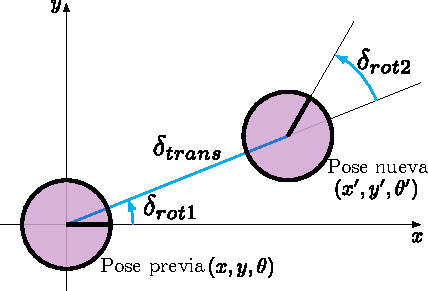
\includegraphics[width=0.5\textwidth]{./images/odometry_as_controls.pdf}
    \caption{Modelo de movimiento.}
    \label{fig:odometry-base-motion-model}
\end{figure}

\subsubsection{Motion Model Jacobian}
We will reuse the odometry motion model from HW1 (see Figure \ref{fig:odometry-base-motion-model} and Sec. 5.4 in the book \cite{thrun2005probabilistic}). The state of the robot is its 2D position and orientation: $s_{t}=[x_{t},y_{t},\theta_{t}]$. The control to the robot is $u_{t}=[\delta_{rot1},\delta_{trans},\delta_{rot2}]$, i.e. the robot rotates by $\delta_{rot1}$, drives straight forward $\delta_{trans}$, then rotates again by $\delta_{rot2}$.

The equations for the motion model $s_{t}=g(u_{t},s_{t-1})$ are as follows:

\begin{align*}
    x_{t} &= x_{t-1}+\delta_{trans}*\cos(\theta_{t-1}+\delta_{rot1}) \\
    y_{t} &= y_{t-1}+\delta_{trans}*\sin(\theta_{t-1}+\delta_{rot1}) \\
    \theta_{t} &= \theta_{t-1}+\delta_{rot1}+\delta_{rot2}
\end{align*}

Your task is to derive the Jacobian matrix $G$, a matrix consisting of the first-order derivative of $s_{t}$ with respect to the previous state $s_{t-1}$, as well as $V$, a matrix consisting of the first-order derivative of $s_{t}$ with respect to the control input $u_{t}$. Since $s_{t},s_{t-1}$ and $u_{t}$ are all 3-dimensional, $G$ and $V$ are both $3\times 3$ matrices.

In short, $s_{t+1}=[x_{t+1},y_{t+1},\theta_{t+1}]$ is the prediction of the motion model. Derive the Jacobians of $g$ with respect to the state $G=\dfrac{\partial g}{\partial s}$ and control $V=\dfrac{\partial g}{\partial u}$:

\[
G=\begin{pmatrix}
\dfrac{\partial x^{\prime}}{\partial x} & \dfrac{\partial x^{\prime}}{\partial y} & \dfrac{\partial x^{\prime}}{\partial \theta} \\
\dfrac{\partial y^{\prime}}{\partial x} & \dfrac{\partial y^{\prime}}{\partial y} & \dfrac{\partial y^{\prime}}{\partial \theta} \\
\dfrac{\partial \theta^{\prime}}{\partial x} & \dfrac{\partial \theta^{\prime}}{\partial y} & \dfrac{\partial \theta^{\prime}}{\partial \theta} \\
\end{pmatrix}
\quad
V=\begin{pmatrix}
\dfrac{\partial x^{\prime}}{\partial \delta_{rot1}} & \dfrac{\partial x^{\prime}}{\partial \delta_{trans}} & \dfrac{\partial x^{\prime}}{\partial \delta_{rot2}} \\
\dfrac{\partial y^{\prime}}{\partial \delta_{rot1}} & \dfrac{\partial y^{\prime}}{\partial \delta_{trans}} & \dfrac{\partial y^{\prime}}{\partial \delta_{rot2}} \\
\dfrac{\partial \theta^{\prime}}{\partial \delta_{rot1}} & \dfrac{\partial \theta^{\prime}}{\partial \delta_{trans}} & \dfrac{\partial \theta^{\prime}}{\partial \delta_{rot2}} \\
\end{pmatrix}
\]

\subsubsection{Observation Model Jacobian}
Assume there is a landmark $m$ at location $(x_{m},y_{m})$. The robot receives two measurements of the bearing angle $\phi$ and the landmark, the range $r$, where

\begin{align*}
    \phi &= \texttt{atan2}(y_{m}-y_{t},x_{m}-x_{t})-\theta_{t} \\
    r &= \sqrt{(x_{m}-x_{t})^{2}+(y_{m}-y_{t})^{2}}
\end{align*}

Derive Jacobian matrix $H_{s}$, derivative of the measurements with respect to the robot state $s_{t}=[x_{t},y_{t},\theta_{t}]$ and the Jacobian matrix $H_{m}$, derivative of the measurements with respect to the landmark position $(x_{m},y_{m})$.

\subsection{EKF Localization and Mapping}
In the programming component of this assignment, you will first implement an Extended Kalman Filter (EKF) (Algorithm~\ref{alg:ekf}) to localize a robot based on landmarks. Then, you will add landmarks to the state and build a map while localizing the robot, thus performing simultaneous localization and mapping (SLAM).

\begin{algorithm}\captionsetup{labelfont={sc,bf}, labelsep=newline}
    \label{alg:ekf}
    \caption{Extended Kalman Filter}
    \begin{algorithmic}[1]
        \Procedure{ExtendedKalmanFilter}{$\mu_{t-1}, \covariance_{t-1}, \controlCommand_{t}, \observation_{t}$}
            \State $\overline{\mu}_{t} = \motionModelFunction{\controlCommand_{t}, \mu_{t-1}}$
            \State $\overline{\covariance}_{t} = \motionModelJacobian_{t} \covariance_{t-1} \motionModelJacobian_{t}^{\top}+\motionParametersCovariance_{t}$
            \Statex
            \State $\kalmanGain_{t} = \overline{\covariance}_{t} \observationModelJacobian_{t}^{\top} (\observationModelJacobian_{t} \overline{\covariance}_{t}  \observationModelJacobian_{t} + \observationModelCovariance_{t})^{-1} $
            \State $\mu_{t} = \overline{\mu}_{t} + \kalmanGain_{t} (\observation_{t} - \observationModelFunction{\overline{\mu}_{t}})$
            \State $\covariance_{t} =  (I - \kalmanGain_{t} \observationModelJacobian_{t}) \overline{\covariance}_{t}$
            \State \Return $\mu_{t}, \covariance_{t}$
        \EndProcedure
    \end{algorithmic}
\end{algorithm}



\subsection*{Code Overview}
The starter code for EKF is under the \texttt{ekf\_slam} folder. The conda environment you installed for HW1 should suffice for this homework.

\subsection*{Command-Line Interface}
First, run \texttt{cd ekf\_slam} to enter the sub-folder. To visualize the robot in the soccer field environment, run:

\begin{verbatim}
$ python localization.py --plot none
\end{verbatim}

The blue line traces out the robot's position, which is a result of noisy actions. The green line traces the robot's position assuming that actions weren't noisy. After you implement a filter, the filter's estimate of the robot's position will be drawn in red.

\begin{verbatim}
$ python localization.py --plot ekf_slam
\end{verbatim}

Typical commands would be like:

\begin{verbatim}
# problem a
$ python localization.py ekf_slam --plot
# problem b
$ python localization.py ekf_slam --multi_run 10 --data-factor 0.1 --filter-factor 0.1
# problem c
$ python localization.py ekf_slam --multi_run 10 --motion-factor 0.1 --observation-factor 1.0
\end{verbatim}

To see other command-line flags available to you, run:

\begin{verbatim}
$ python localization.py -h
\end{verbatim}

\textbf{Hints:}
\begin{itemize}
    \item Make sure to call \texttt{utils.minimized\_angle} any time an angle or angle difference could exceed $[-\pi,\pi]$.
    \item Turn off plotting for a significant speedup.
\end{itemize}

\subsection*{Task}
\begin{enumerate}
    \item Fill in the Jacobian matrices G, V, R and H in \texttt{ekf\_slam.py} using your derivation in 1.1.
    \item Implement the EKF update (Algorithm~\ref{alg:ekf}) in \texttt{ExtendedKalmanFilterSLAM.update} in \texttt{ekf\_slam.py}. Make sure to keep track of the set of landmark IDs that the robot has observed.
\end{enumerate}

Answer the following questions in your writeup:
\begin{enumerate}
    \item Under the default noise parameters, $\alpha=\beta=1$, plot the robot's path and the landmark locations estimated by EKF and compare it with the ground truth path and landmarks.
    \item Plot the position error of the robot state and the landmark positions as the data factor (\texttt{--data-factor}) and the filter noise factor (\texttt{--filter-factor}) vary \textbf{simultaneously} over $[0.01,0.03,0.1,0.3,1.0]$. Keep \texttt{data-factor == filter-factor}, so there are 5 data points. For each data point, run 10 trials with different random seeds (\texttt{--multi\_run 10}) and plot the mean and standard deviation. Does EKF estimate the map accurately? Discuss anything interesting you observe.
    \item Plot the position error of robot state and the landmark positions as the motion factor (\texttt{--motion-factor}) and observation factor (\texttt{--observation-factor}) vary \textbf{independently} over $[0.1,0.3,1.0]$. There are 9 data points in total. Run 10 trials per value with different random seeds (\texttt{--multi\_run 10}) and plot the mean and standard deviation. Discuss anything interesting you observe.
\end{enumerate}

\section{Submission}
We will be using the Canvas for submission of the assignments. Please submit the written assignment answers as a PDF. For the code, submit a zip file of the entire working directory.

\printbibliography

\end{document}